\documentclass[11pt,a4paper]{article}

\usepackage{scribe}

\setseriestitle{Statistical and Algorithmic Learning Theory}
\setscribecode{3}
\setauthname{Gurpreet Singh}
\setinstrname{Purushottam Kar}
\setauthemail{guggu@iitk.ac.in}
\settitle{Parametric Learning in Realizable Settings}

\begin{document}
\makeheader%

Before we attempt to solve a machine learning problem, we must accurately define the model or setting. Hence, we first define a formal model aimed to cover learning tasks.

We only cover parametric learning models \et{e.g.} Binary Classification, Regression, etc in this chapter and following ones

\begin{ssection}{Definition of a Formal Model and Notations}

	\begin{enumerate}[label=\bt{\theenumi.}]
		\ditem[Instance/Feature Space] ($\cX$) --- This is the space of the random variable that defines the data distribution. $\cX$ is the set of objects that we wish to label. For example, for the problem of classifying an email as spam or not-spam, the set of emails defines the set $\cX$ \sbr

		\ditem[Output Space] ($\cY$) --- This defines the space of the random variable that is the label or value mapped to each data point. For example, in the problem of email classification, the output space is $\set{0, 1}$ where 1 is for spam and 0 for not-spam. There can be different Output Spaces depending on the problem.

			\begin{itemize}[label=-\;]
				\item Labeling: $\set{-1, 1}, \bR^p$
				\item Permutation: $S_n$
				\item Hierarchy / Tree
				\item Alternate Representation: $\bR^D \ra \bR^d$ (\et{e.g.} Dimensionality Reduction)
			\end{itemize} \sbr

		\ditem[Distribution] ($\cD$) --- This is also known as the data generation distribution. $\cD$ defines the probability distribution of the data points (and sometimes also labels, more in agnostic setting). For the realizable setting, this distribution is used to sample data points say $\set{x^1, x^2 \dots x^n}$ and a \et{prediction rule} $f : \cX \ra \cY$ is used to map the data points to their respective labels, as per defined by the prediction rule \et{i.e.} $y^i = f(x^i)$

		\ditem[Training Sample] ($S$) --- This is a tuple or sequence of $n$ data points and their mapped label/parameter sampled from the \et{distribution} or are randomly obtained. $S = \para{\para{x^1, y^1}, \para{x^2, y^2} \dots \para{x^n, y^n}} \in (\cX \times \cY)^n$. This is the part of data that is generally visible to us, and is used for learning prediction models.

		\ditem[Loss Function] ($l$) --- Loss function defines the similarity / dissimilarity in the estimated label value and the actual / observed label value. We say $l : (f(\cX), \cY) \ra \bR$. There are different types of loss functions, for example the squared loss function $l^{\mt{sq}}$ and the 0 -- 1 loss function $l^{0-1}$.

		\ditem[Algorithm] ($A$) --- We say that the algorithm maps the generated / sampled training sample to a function belonging in the hypothesis space \et{i.e.}

			\begin{align*}
				A :& \,S \mapsto \hat{f}_s \in \cH \\
				A :& \bigcup_{n = 1}^\infty (\cX, \cY)^n \mapsto \cH
			\end{align*}

		\ditem[l-risk] ($\err[_D^l]{f}$) --- This is defined as the expected loss/error that is obtained for a function $f$ given a loss function $l : (f(\cX), \cY) \ra \bR$.
			\begin{align*}
				\err[_D^l]{f}	\qdeq	\E[(x, y) \sim D]{l(f(x), y)}
			\end{align*}

		\ditem[emperical risk] ($\err[_D^l]{f}$) --- This is defined as the weighted loss/error on the training sample that is obtained for a function $f$ given a loss function $l : (f(\cX), \cY) \ra \bR$
			\begin{align*}
				\err[_S^l]{f}	\qdeq	\frac{1}{n} \sum_{i = 1}^n l(f(x^i), y^i)
			\end{align*}

	\end{enumerate} \sbr

	\begin{exercise}
		Show that $\err[_D^l]{f} = \E{\err[_S^l]{f}}$
	\end{exercise} \sbr

	\begin{exercise}
		Show that $\err[_D^{l^{0-1}}]{f} = \err[_S^{0-1}]{f}$ where
		\begin{align*}
			l^{0-1}(\hat{y}, y)	\eq	1 - \is{y = \hat{y}}
		\end{align*}
	\end{exercise} \sbr

	\begin{exercise}
		Find out $\err[_D^{l^{0-1}_\alpha}]{f}$ in terms of the empirical risk where
		\begin{align*}
			l^{0-1}_\alpha	\eq	\begin{cases}
				\alpha		&	\hat{y} \ne y, y = 1 \\Â
				1 - \alpha	&	\hat{y} \ne y, y = 0 \\
				0			&	\hat{y} = y
			\end{cases}
		\end{align*} \sbr
	\end{exercise}

\end{ssection}

\begin{ssection}{Empirical Risk Minimization}

	We need to have a learning algorithm to reduce the l-risk / true error on the distribution. However, as discussed earlier, we can only see the training sample $S$, and hence we have no direct way to minimize error on the true distribution (given some loss function) \et{i.e.} $\err[_D^l]{l}$.

	To tackle this, we try to minimize the empirical error or empirical risk. The intuition behind this is the assumption / expectation that the training sample is a snapshot of the true data distribution and it explains the universe well.

	Hence, our learning algorithm gives us a prediction rule $\hat{f} \in \cH$ which is the estimate of the true $f^\ast$ where
	\begin{align*}
		f^\ast					&\eq	\argmin{f} \err[_D^l]{f} \\
		f^\ast \qapprox f_{ERM}	&\eq	\argmin{f \in \cH} \err[_S^l]{f}
	\end{align*}

	Although we have a nice prediction rule which allows us to learn our sample training, and is expected to be a good predictor for the complete data / universe as well. However, the ERM predictor may highly overfit the sample training data.

	\begin{ssubsection}{Overfitting of Training Sample}

		To understand what overfitting is, let us take a simple binary classification example.

		\begin{figure}[h!]
			\centering
			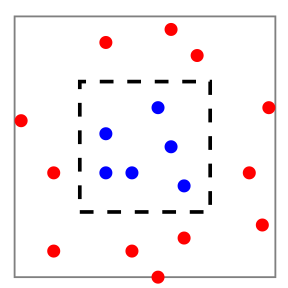
\includegraphics[height=100px]{includes/overfitting-example.png}
			\caption{Randomly sampled data points with red / blue labels. Figure taken from \cite{ml-tta}}
			\label{fig:overfitting}
		\end{figure}

		Suppose we have some data points (universe) sampled randomly within a box, as shown in Figure \ref{fig:overfitting}. Also, for some $S$, the sampled data points for the training sample are the points within the gray box.

		Therefore, we can write a prediction rule which always labels the data point as 1. Since this gives training error as 0 \et{i.e.} $\err[_S^l]{f} = 0$. However, the same prediction rule gives high error when run on the complete data.

		Therefore, a predictor that performs ``too well'' on a training sample, whereas gives a high error on the complete data is said to \et{overfit} the data. We can also write the formal definition of overfitting.

		\begin{definition}[Overfitting \citep{oxford-overfitting}]
			The production of an analysis which corresponds too closely or exactly to a particular set of data, and may therefore fail to fit additional data or predict future observations reliably.
		\end{definition}

	\end{ssubsection}

	\begin{ssubsection}{Empirical Risk Minimization with Inductive Bias}

		We know that the ERM method might lead to overfitting. In order to avoid that, we need to understand the reason behind it.

		The overfitting problem is caused by the learner fitting a function to accurately predict the labels for all the data points in the training sample. Hence, rather than predicting the general pattern in the data.

		A simple solution to this is to restrict the search space of the prediction function. Hence, instead of minimizing the empirical risk over all functions, we will look at only a set of possible functions. This set is called the \et{hypothesis class} or the \et{model class} (or \et{hypothesis space}). We can formally define this as below.

		\begin{definition}[Hypothesis/Model Space]
			The hypothesis class (represented as $\cH$) defines the set of all functions $\set{f : \cX \ra \cY}$ belonging to a certain function class, for example for a regression case, the hypothesis space can be all the linear functions passing through $\vzero$. Since this is the set of different mappings (prediction rules) of all data points, we can say $\cH \subseteq \cY^\cX$.
		\end{definition}

		Therefore, we now redefine the ERM model to learn a predictor belonging to the hypothesis class only.
		\begin{align*}
			\hat{f}	\eq	\argmin{f \in \cH} \err[_D^l]{f}
		\end{align*}

		Such restrictions, for exampling, fixing the hypothesis space is called the \et{inductive bias}.

	\end{ssubsection}

	\begin{ssubsection}{Avoiding Overfitting with Finite Hypothesis Spaces}

		We claimed in the previous section that we can avoid overfitting if we use Hypothesis space. However, overfitting is highly probably avoided in case of finite hypothesis spaces. More formally, if the hypothesis space $\cH$ is a finite class of size $m$, where $m$ is \et{sufficiently large}, then the risk of the predictor function is bounded with a high probability.

		\note{We will prove this for the realizable setting, however this also holds for the agnostic setting as well, but only the bounds will change by a constant term, as we will see later.}

		We still need to define when is $m$ ``sufficiently large'', however, first we need to take some generic assumptions for our model.

		\begin{enumerate}[label=\bt{\theenumi.}]
			\ditem[Indepent and Identically Distributed Assumption.] This assumption states that the data points in the training sample are independent and identically distributed according to the distribution $\cD$. Therfore, $S$ is essentially a set of $n$ independent data points all sampled from $\cD$. We represent this as $S \iid \cD^n$.
			\ditem[The Realizability Assumption.] The realizability assumption states that there exists $f^\ast \in \cH$ such that $\err[_D^l]{f^\ast} = 0$. This assumption says that the with probability 1 over any random sample, $S$, $\err[_S^l]{f^\ast}$
		\end{enumerate}

		Since $S$ is sampled using the data distribution, $\cD$, we can say that $S$ and therefore $\err[_S^l]{f}$ are random variables for some $f \in \cH$. We say an algorithm for a learning model is very less likely to overfit if the l-risk for all functions learned by the algorithm for any sample is bounded by $\epsilon$ with probability more than $1 - \delta$ where $\epsilon$ is the accuracy parameter and $\delta$ is the confidence parameter.

		Therefore, we need to bound $\prob{\err[_D^l]{f_S} > \epsilon}$. Since this is just dependent on $S$, we can write this in an alternate way
		\begin{align*}
			\prob{\err[_D^l]{f_S} > \epsilon}	\eq	\cD^m \para{S \pipe \err[_D^l]{f_S} > \epsilon}
		\end{align*} \sbr

		Hence, we want to bound $\cD^m \para{S \pipe \err[_D^l]{f_S} > \epsilon}$. We can define a few more terms, which will make the proof easier.

		\begin{align*}
			\cH_B	&\eq	\set{f \in \cH \pipe \err[_D^l]{f} > \epsilon} \\
			M		&\eq	\set{S \pipe \qexists f \in \cH, \err[_S^l]{f} = 0}
		\end{align*} \sbr

		where $\cH_B$ defines the set of (bad) functions which give l-risk more than $\epsilon$ and $M$ as the set of (misleading) samples for which there is at least one function which gives 0 empirical risk. We say that we are misleaded only when our sample gives 0 empirical risk, but high l-risk \et{i.e.} the set of samples that give a bad hypothesis (prediction function) must a subset of the misleading samples. Therefore,
		\begin{align*}
			\set{S \pipe \err[_D^l]{f_S} > \epsilon}				&\qsubseteq	M
			\implies \cD^m\para{S \pipe \err[_D^l]{f} > \epsilon}	&\qle		\cD^m\para{M}
		\end{align*} \sbr

		We can also rewrite $M$ as
		\begin{align*}
			M	\eq	\bigcup_{f \in \cH} \set{S \pipe \err[_S^l]{f} = 0}
		\end{align*} \sbr

		Substituting the above form of $M$ in the previous equation and using the union bound, we get
		\begin{align*}
			\cD^m\para{S \pipe \err[_D^l]{f} > \epsilon}	&\qle		\sum_{f \in \cH} \cD^m\para{\set{S \pipe \err[_S^l]{f} = 0}}
		\end{align*} \sbr

		wher $f \in \cH_B$ is some fixed bad prediction rule. Since the sample is generated i.i.d., , we can write
		\begin{align*}
			\func{\cD^m}{\set{S \pipe \err[_S^l]{f} = 0}}	&\eq	\func{\cD^m}{\set{S \pipe \qforall i, f(x^i) = y^i}} \\
															&\eq	\prod_{i = 1}^n \func{\cD}{\set{x^i \pipe f(x^i) = y^i}} \\
															&\eq	\prod_{i = 1}^n 1 - \err[_D^l]{f} \\
															&\qle	\para{1 - \epsilon}^n \\
															&\qle	\exp{-\epsilon n}
		\end{align*} \sbr

		Hence, we can combine all the equations and write
		\begin{align*}
			\func{\cD^m}{\set{S \pipe \err[_D^l]{f_S} > \epsilon}}	\qle	\abs{\cH_B} \exp{-\epsilon n}	\qle	\abs{\cH} \exp{-\epsilon n}
		\end{align*} \sbr

		We can now define the bound on the size of the training sample $S$

		\begin{theorem}
			For some finite hypothesis class, $\cH$, let $\delta, \epsilon \in \para{0, 1}$ and let $m$ be an integer that satisfies
			\begin{align*}
				m	\qge	\frac{\log{\abs{\cH} / \delta}}{\epsilon}
			\end{align*}
			Then for any prediction function $f$, and for any distribution $\cD$, for which the realizability assumption holds, with probability of at least $1 - \delta$ over the choice of an i.i.d. sample $S$ of size $m$, we have that for every ERM hypothesis class will be probably (with confidence $1 - \delta$) approximately (up to an error $\epsilon$) correct.
		\end{theorem}

	\end{ssubsection}

\end{ssection}

\bibliography{scribes}
\bibliographystyle{plainnat}

\end{document}
